\subsection{Direct triangles and refined native choices}
\label{sec:triangle-results}
We freeze the added formula and cost policy before testing 40 new requests. Twenty contain native two- or three-loop reductions, and twenty contain single triangles or independent triangle products. The product tests cover every loop order from one through thirteen. We measure three fresh-process repetitions for each request and method. These first measurements retain the original runtime monitor. The preceding application, the new fixed control, and the new integrated method receive the same physical inputs. Times include application loading, model use where enabled, algebra, output reading, and cleanup. Independent coefficient comparisons remain outside all timers.

\begin{table}[htbp]\centering\small
\caption{New reserved requests. Times sum per-request medians of three complete calls. The ratio divides new time by preceding time.}
\label{tab:triangle-times}
\begin{tabular}{lrrrr}\toprule
Requests & Number & Preceding (s) & New (s) & Ratio\\\midrule
One-scale triangles and products & 20 & 5.231 & 4.269 & 0.816 \\
Planar boxes & 5 & 10.829 & 8.792 & 0.812 \\
Nonplanar boxes & 5 & 17.214 & 13.123 & 0.762 \\
Massive sunrise & 5 & 10.215 & 10.265 & 1.005 \\
Three-loop vacuum & 5 & 14.277 & 14.399 & 1.009 \\
\bottomrule\end{tabular}\end{table}

The native requests give a total-time ratio of 0.887, with a paired request-bootstrap interval of $[0.743,1.010]$. The integrated-to-fixed ratio is 1.010, with interval $[0.990,1.029]$. Both new methods use the same fixed choices because the added selector is disabled. Their timing difference does not measure a new ML gain.
 The seven-loop product request has a time ratio of 1.077 in this fresh-process comparison. The measurements therefore include a slower triangle case, and they do not establish a monotonic trend with loop order.

\begin{figure}[htbp]\centering
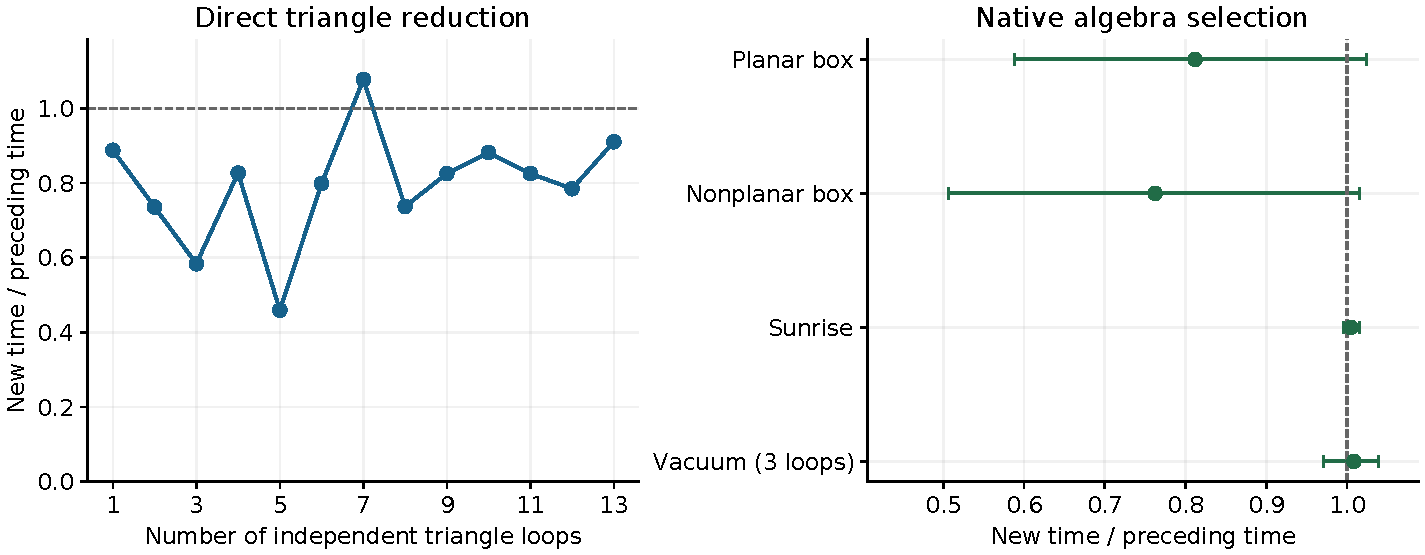
\includegraphics[width=\linewidth]{paper_figures/triangle_extension.pdf}
\caption{Complete-time ratios on the new requests. The dashed line marks equal time. The left panel shows the direct triangle implementation at each tested product loop order. The right panel shows native requests by propagator structure, with paired request-bootstrap intervals. Product tests do not establish connected higher-loop scattering performance.}
\label{fig:triangle-extension}
\end{figure}

\subsection{Final complete-call comparison}
A native reduction removes temporary files while it runs. The earlier resource monitor could stop a reduction if a directory disappeared during its inspection. We change the monitor to tolerate removal while preserving its storage bound. A controlled check reproduces the old exception and verifies the new behavior. This change affects runtime supervision and leaves the algebra and learned decisions unchanged.

We compare the preceding published application, the new mathematical method with the original monitor, and the final application with the corrected monitor on the same 93 requests. Each method runs three times on the same compute node with one worker, rotating method order, and reversed request order in the middle repetition. A preceding two-worker comparison showed timing differences larger than the measured monitor cost. It also stopped when recovery in the preceding application returned a 20-integral basis instead of the 16-integral reference basis for one vacuum request. We retain that failed comparison separately. The complete serial check uses every planned request and method. The complete timer includes unsuccessful internal attempts and recovery. Independent comparisons check the saved exact coefficients outside the timer.
\begin{table}[htbp]\centering\small
\caption{Final matched shared-call comparison. Times are complete collection times. The range shows the three observations. Internal failures count attempts across all three repetitions.}
\label{tab:triangle-final}
\begin{tabular}{lrrrr}\toprule
Method & Median (s) & Mean (s) & Range (s) & Failures\\\midrule
Preceding application & 45.091 & 45.230 & 44.783--45.817 & 0 \\
New method, original monitor & 42.932 & 42.624 & 40.351--44.589 & 0 \\
Final application & 41.137 & 41.029 & 40.723--41.227 & 0 \\
\bottomrule\end{tabular}\end{table}
The final-to-preceding median ratio is 0.912, which reduces time by 8.8 percent on this collection. The final-to-original-monitor ratio is 0.958. All 837 application results pass 13,401 exact coefficient comparisons. This finite timing comparison does not prove a universal speedup or a globally shortest reduction.
